Chương này trình giải pháp cho bài toán đa robot phối hợp đẩy vật, chia ra làm hai pha là pha khám phá - nơi robot chưa thực hiện nhiệm vụ ngay mà sẽ tiến hành và pha đẩy vật khi robot bắt đầu thực hiện nhiệm vụ. Ba bài toán lớn cần được giải quyết lần lượt là ước lượng vị trí điểm trọng tâm trong pha khám phá, xây dựng đội hình đa robot và lên chiến thuật đẩy trong pha đẩy vật.
\section{Mô hình hóa hệ thống}
Trong đồ án này robot được biểu diễn dưới dạng chất điểm hình tròn bán kính $r_r$, được trang bị cảm biến lực có khả năng đo lực pháp tuyến. Robot có khả năng di chuyển về mọi hướng, có khả năng tương tác với vật thể thông qua tương tác đẩy với lực pháp tuyến nằm trong khoảng từ $[0 , f_\text{max}]$. Giả định các robot có khả năng duy trì tương tác với vật thể tại điểm tương tác (contact point) tại mọi thời điểm. Vật thể đươc mô hình hóa dưới dạng một khối vật rắn (rigid body) có hình dạng đa giác, có khối lượng $m$ và quán tính $I$, khối tâm tại $C$.   
\section{Không gian làm việc}
Do vị trí các robot cần được đặt sao cho cảm biến ở rìa của robot phải ở trên cạnh của vật, hay nói cách khá là vị trí của robot chỉ chạy xung quanh biên hình học của vật nên thay vì phải tìm kiếm trong không gian 2D, không gian vị trí của các robot được nén xuống một miền không gian 1 chiều, gọi là $U$.
\begin{figure}[H]
    \centering
    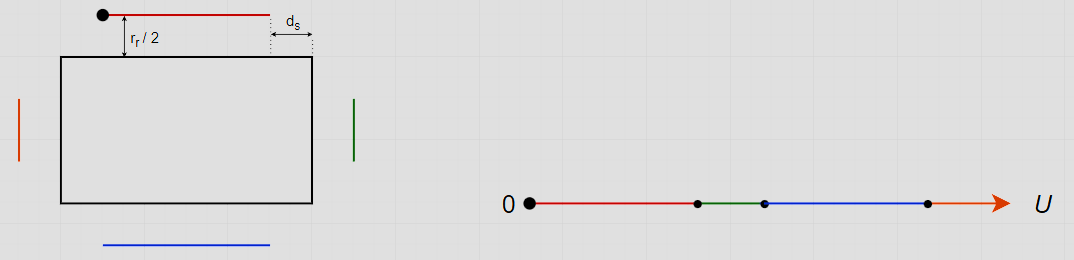
\includegraphics[scale=0.51]{chapter5/image/U.png}
    \caption{Cách xây dựng không gian làm việc $U$}
    \label{fig:U}
\end{figure}
Để xác định được miền $U$, đầu tiên ta vẽ lại các cạnh của vật thể, sau đó dịch các cạnh đó song song với cạnh gốc đi một khoảng $\frac{r_r}{2}$, đúng bằng khoảng cách từ tâm đến biên của robot. Với đa giác không lồi, các cạnh này có thể cắt nhau, khi đó ta bỏ phần giao nhau này đi. Các cạnh này sau đó được cắt ngắn đi 2 đầu một khoảng $d_\text{s}$, được gọi là khoảng cách an toàn đỉnh, do ta không muốn các robot ở quá gần các đỉnh của vật, khi này ta có một tập cạnh $E$. Chọn một điểm bất kỳ ở đầu một trong các đoạn thẳng trong tập $E$ làm gốc tọa độ, có thể chọn bằng cách sắp xếp theo tọa độ x,y so với hệ quy chiếu gắn với vật và lấy bé nhất, sau đó các ghép lần lượt các đoạn thẳng trong tâp $E$ nối đuôi nhau bắt đầu từ đoạn thẳng chứa đỉnh gốc theo chiều kim đồng hồ thành một đường thẳng duy nhất, đó chính là miền $U$ như hình \ref{fig:U}. Khi này vị trí của các robot sẽ được mô tả qua miền miền U, vị trí tương ứng của nó khi tác dụng lực lên vật trên không gian 2D sẽ có thể có được bằng một hàm $p(u)$ với $u \in U$.
\section{Ước lượng trọng tâm}
Trong pha khám phá, bầy robot sẽ tiến hành quá trình khám phá nhằm thu thập các thông tin về vật trước khi bắt đầu quá trình, trong đó thông tin về hình dạng của vật được giả định là đã có được thông qua một trong các phương pháp được nêu ở chương \ref{sec:pushing}, ví dụ như lấy thông tin từ camera nhìn từ trên xuống. Do đó phần này chủ yếu trình bày quy trình trong phương pháp ước lượng các thông tin về trọng tâm của vật dựa trên gia tốc góc thông qua các lần đẩy thử. Mỗi robot sẽ lần lượt thực hiện khám phá để có được thông tin này.

\subsection{Phương pháp ước lượng}
Dựa vào tính chất cơ bản của điểm trọng tâm, lực tác dụng vuông góc với 1 cạnh đa giác tại đúng hình chiếu của trọng tâm lên cạnh đó sẽ không sinh ra mô men xoay, vị trí điểm trọng tâm trên vật có thể được xác định khi ta có ít nhất hai hình chiếu của nó lên hai cạnh bất kỳ không song song bằng cách lấy giao của hai vector pháp tuyến như hình \ref{fig:COM}.
\begin{figure}[H]
    \centering
    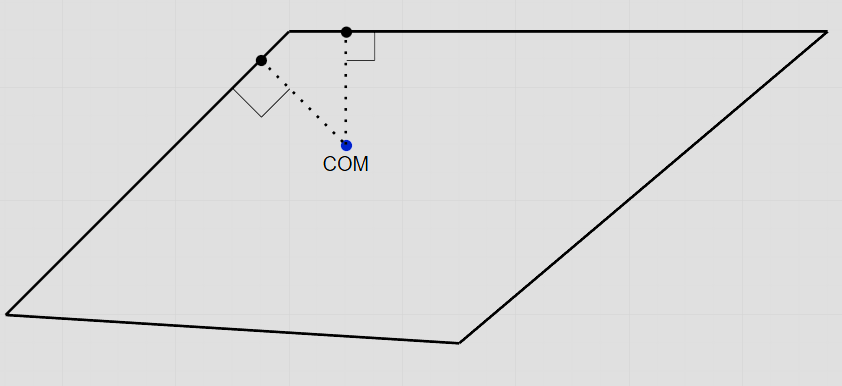
\includegraphics[scale=0.5]{chapter5/image/com.png}
    \caption{Trọng tâm được xác định khi biết hình chiếu lên hai cạnh}
    \label{fig:COM}
\end{figure}

Lúc này bài toán trở thành việc ước lượng vị trí hình chiếu của trọng tâm lên cạnh của vật thông qua phương pháp đẩy thử. Với đa giác không lồi thì có nhiều trường hợp mà hình chiếu của trọng tâm lên cạnh đang xét sẽ nằm ngoài cạnh hoặc vùng được chuyển sang miền $U$, do đó robot không thể đẩy tại điểm này. Đồ án đề xuất một cách tiếp cận không cần tác dụng lực đẩy đi qua điểm trọng tâm, đó là xét yếu tố gia tốc góc. Khác với gia tốc tịnh tiến, gia tốc góc của vật có thể được đo ngay cả khi ta chưa biết điểm trọng tâm bằng cách theo dõi ít nhất 2 điểm quy chiếu bất kỳ trên vật, hay trong bài toán này có thể đo lường gián tiếp thông qua gia tốc góc của robot, vì ta giả định robot luôn duy trì được lực đẩy vuông góc với cạnh tiếp xúc. Thuật toán dựa trên công thức \ref{eq:ang} để xây dựng hệ phương trình, sau đó giải để tìm vị trí của hình chiếu. 

\subsection{Xây dựng hệ phương trình}

Tại một cạnh bất kỳ của vật thể ta cho robot đẩy lần lượt tại ba vị trí khác nhau $[u_i]_{i=1}^{3} \in U$ , với ba lực đẩy có độ lớn khác nhau $[f_i]_{i=1}^{3} \in R$ với thỏa mãn điều kiện là các lực đẩy vuông góc với cạnh và sinh ra chuyển động quay. Gọi độ dài cánh tay đòn tại ba điểm này lần lượt là $r_0$,  $r_0 + \Delta r_1$ và $r_0 + \Delta r_2$, trong đó $r_0 = lv(u_1) \in R$ với $lv$ là hàm để lấy cánh tay đòn tương ứng theo vị trí trong $U$ Dựa vào công thức \ref{eq:ang}, ta có hệ phương trình bậc nhất với 3 ẩn là đô dài cánh tay đòn $r_0$, độ lớn mô men ma sát $\tau_{fr}$ và quán tính $I$ như sau:
\begin{equation}
\label{eq:eq3}
\begin{cases}
f_1 \, r_0 - \operatorname{sgn}(\dot{\theta_1})\,\tau_{fr} -  {\ddot{\theta}}_1 \,I = 0\\
f_2 \, r_0 - \operatorname{sgn}(\dot{\theta_2})\,\tau_{fr} -  {\ddot{\theta}}_2 \,I = - f_2 \, \Delta r_1\\
f_3 \, r_0 - \operatorname{sgn}(\dot{\theta_3})\,\tau_{fr} -  {\ddot{\theta}}_3 \,I = - f_3 \, \Delta r_2
\end{cases}
\end{equation}
trong đó các giá trị về gia tốc góc $\ddot{\theta}_i$ được đo bởi robot trong mỗi lần đẩy.

Hệ phương trình \ref{eq:eq3} có nghiệm duy nhất khi và chỉ khi định thức của nó khác không hay:
\begin{equation}
\operatorname{sign}(\dot\theta_{1})\big(\ddot\theta_{2}f_{3}-\ddot\theta_{3}f_{2}\big)
+ \operatorname{sign}(\dot\theta_{2})\big(\ddot\theta_{3}f_{1}-\ddot\theta_{1}f_{3}\big)
+ \operatorname{sign}(\dot\theta_{3})\big(\ddot\theta_{1}f_{2}-\ddot\theta_{2}f_{1}\big) \ne 0
\end{equation}

\begin{figure}[H]
    \centering
    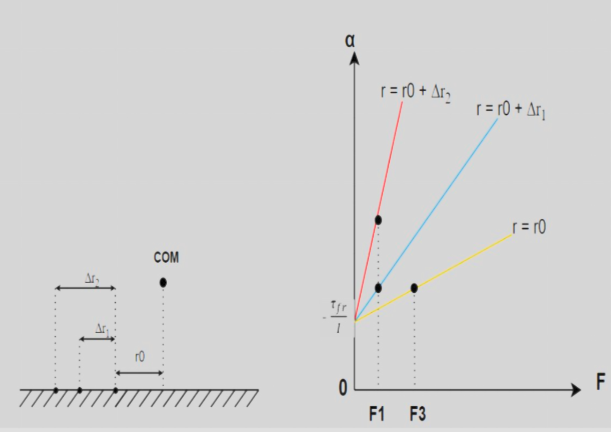
\includegraphics[scale=0.5]{chapter5/image/phi.png}
    \caption{Một cách chọn lực đẩy để hệ không suy biến}
    \label{fig:phi}
\end{figure}

Với trường hợp tất cả các vị trí đẩy cùng chiều cánh đòn, điều kiện cần và đủ là các điểm ($f_1 , {\ddot{\theta}}_1$), ($f_2 , {\ddot{\theta}}_2$) và ($f_3 , {\ddot{\theta}}_3$) không nằm trên một đường thẳng, điều này có thể dễ dàng đạt được nếu ta chọn vị trí đẩy khác nhau và lực đẩy hợp lý do gia tốc góc và lực đẩy với các cánh tay đòn khác nhau vốn không cùng tỷ lệ, một cách chọn để chắc chắn là chọn $f_1 = f_2 \ne f_3$ như trong hình (\ref{fig:phi}), tương tự với trường hợp khác chiều ta cũng có thể lựa chọn lực phù hợp để đảm bảo hệ không suy biến. 
Giải hệ phương trình \ref{eq:eq3} ta thu được độ dài cánh tay đòn tương ứng với vị trí $u_i$ là $r_0$, từ đó ta tìm được hình chiếu $C'$ của $C$ trên cạnh đang xét do ta biết chiều quay của mô men. Với số lần đẩy tối thiểu trên mỗi cạnh là 3 và số cạnh tối thiểu cần xét là 2, robot cần tối thiểu 6 lần đẩy - một con số khá thấp để có thể ước lượng được vị trí điểm trọng tâm của vật.

\subsection{Phương pháp bình phương tối thiểu}
Trong trường hợp cảm biến có nhiễu, hay đơn giản là muốn tăng số mẫu thu thập lên để nâng độ tin cậy về thông tin, ta hoàn toàn có thể đẩy nhiều hơn 3 lần thử với mỗi cạnh, khi này hệ \ref{eq:eq3} trở thành:
\begin{equation}
\begin{cases}
\label{eq:eq3p}
f_1 r_0 - \operatorname{sgn}(\dot{\theta_1})\,\tau_{fr} - \ddot{\theta}_1 I = 0\\[3pt]
f_2 r_0 - \operatorname{sgn}(\dot{\theta_2})\,\tau_{fr} - \ddot{\theta}_2 I = -f_2 \Delta r_1\\[3pt]
\vdots\hspace{4cm}\vdots \\[3pt]
f_n r_0 - \operatorname{sgn}(\dot{\theta_n})\,\tau_{fr} - \ddot{\theta}_n I = -f_n \Delta r_{n-1}
\end{cases}
\end{equation}

Mỗi phương trình trong \ref{eq:eq3p} có dạng:
\begin{equation}
\label{eq:ln}
    f_i r_0 - \operatorname{sgn}(\dot{\theta_i})\,\tau_{fr} - \ddot{\theta}_i I = b_i,
\end{equation}

\begin{equation}
    b_i =
    \begin{cases}
        0, & i = 1,\\[4pt]
        - f_i \Delta r_{i-1}, & i = 2, \ldots, n.
    \end{cases}
\end{equation}

Do đó về mặt bản chất, bài toán trở thành một bài toán hồi quy tuyến tính (linear regression) cho hàm \ref{eq:ln}. Hệ phương trình~\ref{eq:eq3p} có thể được viết gọn dưới dạng ma trận $A x = b$ với:
\begin{equation}
A =
\begin{bmatrix}
f_1 & -\operatorname{sgn}(\dot{\theta_1})\, & -\ddot{\theta}_1\\
f_2 & -\operatorname{sgn}(\dot{\theta_2})\, & -\ddot{\theta}_2\\
\vdots & \vdots & \vdots\\
f_n & -\operatorname{sgn}(\dot{\theta_n})\, & -\ddot{\theta}_n
\end{bmatrix},
\quad
x =
\begin{bmatrix}
r_0\\[3pt]
\tau_{fr}\\[3pt]
I
\end{bmatrix},
\quad
b =
\begin{bmatrix}
0\\[3pt]
-f_2 \Delta r_1\\[3pt]
\vdots\\[3pt]
-f_n \Delta r_{n-1}
\end{bmatrix}.
\end{equation}

Do khi $n > 3$, hệ dư phương trình, không có nghiệm đúng tuyệt đối, ta sử dụng phương pháp bình phương tối thiểu để tìm nghiệm có sai số bình phương nhỏ nhất $x^{*} = \arg\min_x \|A x - b\|^2$ bằng cách giải: 
\begin{equation}
    x^{*} = (A^{\mathrm{T}} A)^{-1} A^{\mathrm{T}} b
\end{equation}

\subsection{Khả năng mở rộng}
Dù cho vốn được thiết kế để từng robot tiến hành khám phá lần lượt, phương pháp đề xuất hoàn toàn có thể được áp dụng, thậm chí là được khuyến khích sử dụng với bài toán nhiều robot trong mỗi lần đẩy. Tuy phải chấp nhận yếu tố về truyền thông, phương pháp này lại có những ưu điểm vượt trội so với khi chỉ sử dụng đơn robot. Đầu tiên, nó có thể giải quyết vấn đề khi một đơn vị robot độc lập không sinh đủ lực để thắng lực ma sát tĩnh, làm vật đứng yên mà không di chuyển. Quan trọng hơn, nhờ việc tăng cường số robot trong mỗi lần đẩy nhằm tăng lực tối đa của mỗi cú đẩy có thể khiến cho chênh lệch về lực $f_i$ và gia tốc góc $\ddot{\theta}_i$ trở nên lớn hơn, tránh trường hợp hệ suy biến. Ngoài ra thì việc tăng số robot trong một lượt đẩy cùng cơ chế truyền thông cũng giúp các robot chia sẻ thông tin lúc đẩy với nhau, giảm đáng kể thời gian chờ đợi.




